\part{DPaper -- Papier als digitales Speichermedium}
\ppartpage{von Lars Stoltenow}

\section{Einführung}

\subsection{Worum geht's (nicht)?}
\begin{frame}[<+->]{Worum geht's (nicht)?}
	\begin{itemize}
	\item Vielzahl von Backupmedien
	\item DVDs, Festplatten, Flash, Magnetband
	\item Warum nicht mal Papier?
	\item Einfach mal Spaß haben, statt etwas Praxistaugliches zu produzieren :-)
	\end{itemize}
\end{frame}

\subsection{Vorteile von Papier als Speichermedium}
\begin{frame}[<+->]{Vorteile von Papier als Speichermedium}
	\pause
	\begin{itemize}
	\item Herkömmliche Speichermedien haben begrenzte Lebensdauer:
		\begin{itemize}
		\item CD, DVD: 5-10 Jahre
		\item Festplatten: 2-10 Jahre
		\item Magnetband: 30 Jahre
		\item Papier: \emph{>100} Jahre
		\end{itemize}
	\item Holz ist ein nachwachsender Rohstoff
	\end{itemize}
\end{frame}

\subsection{Funktionsweise}
\begin{frame}{Funktionsweise}
	\pause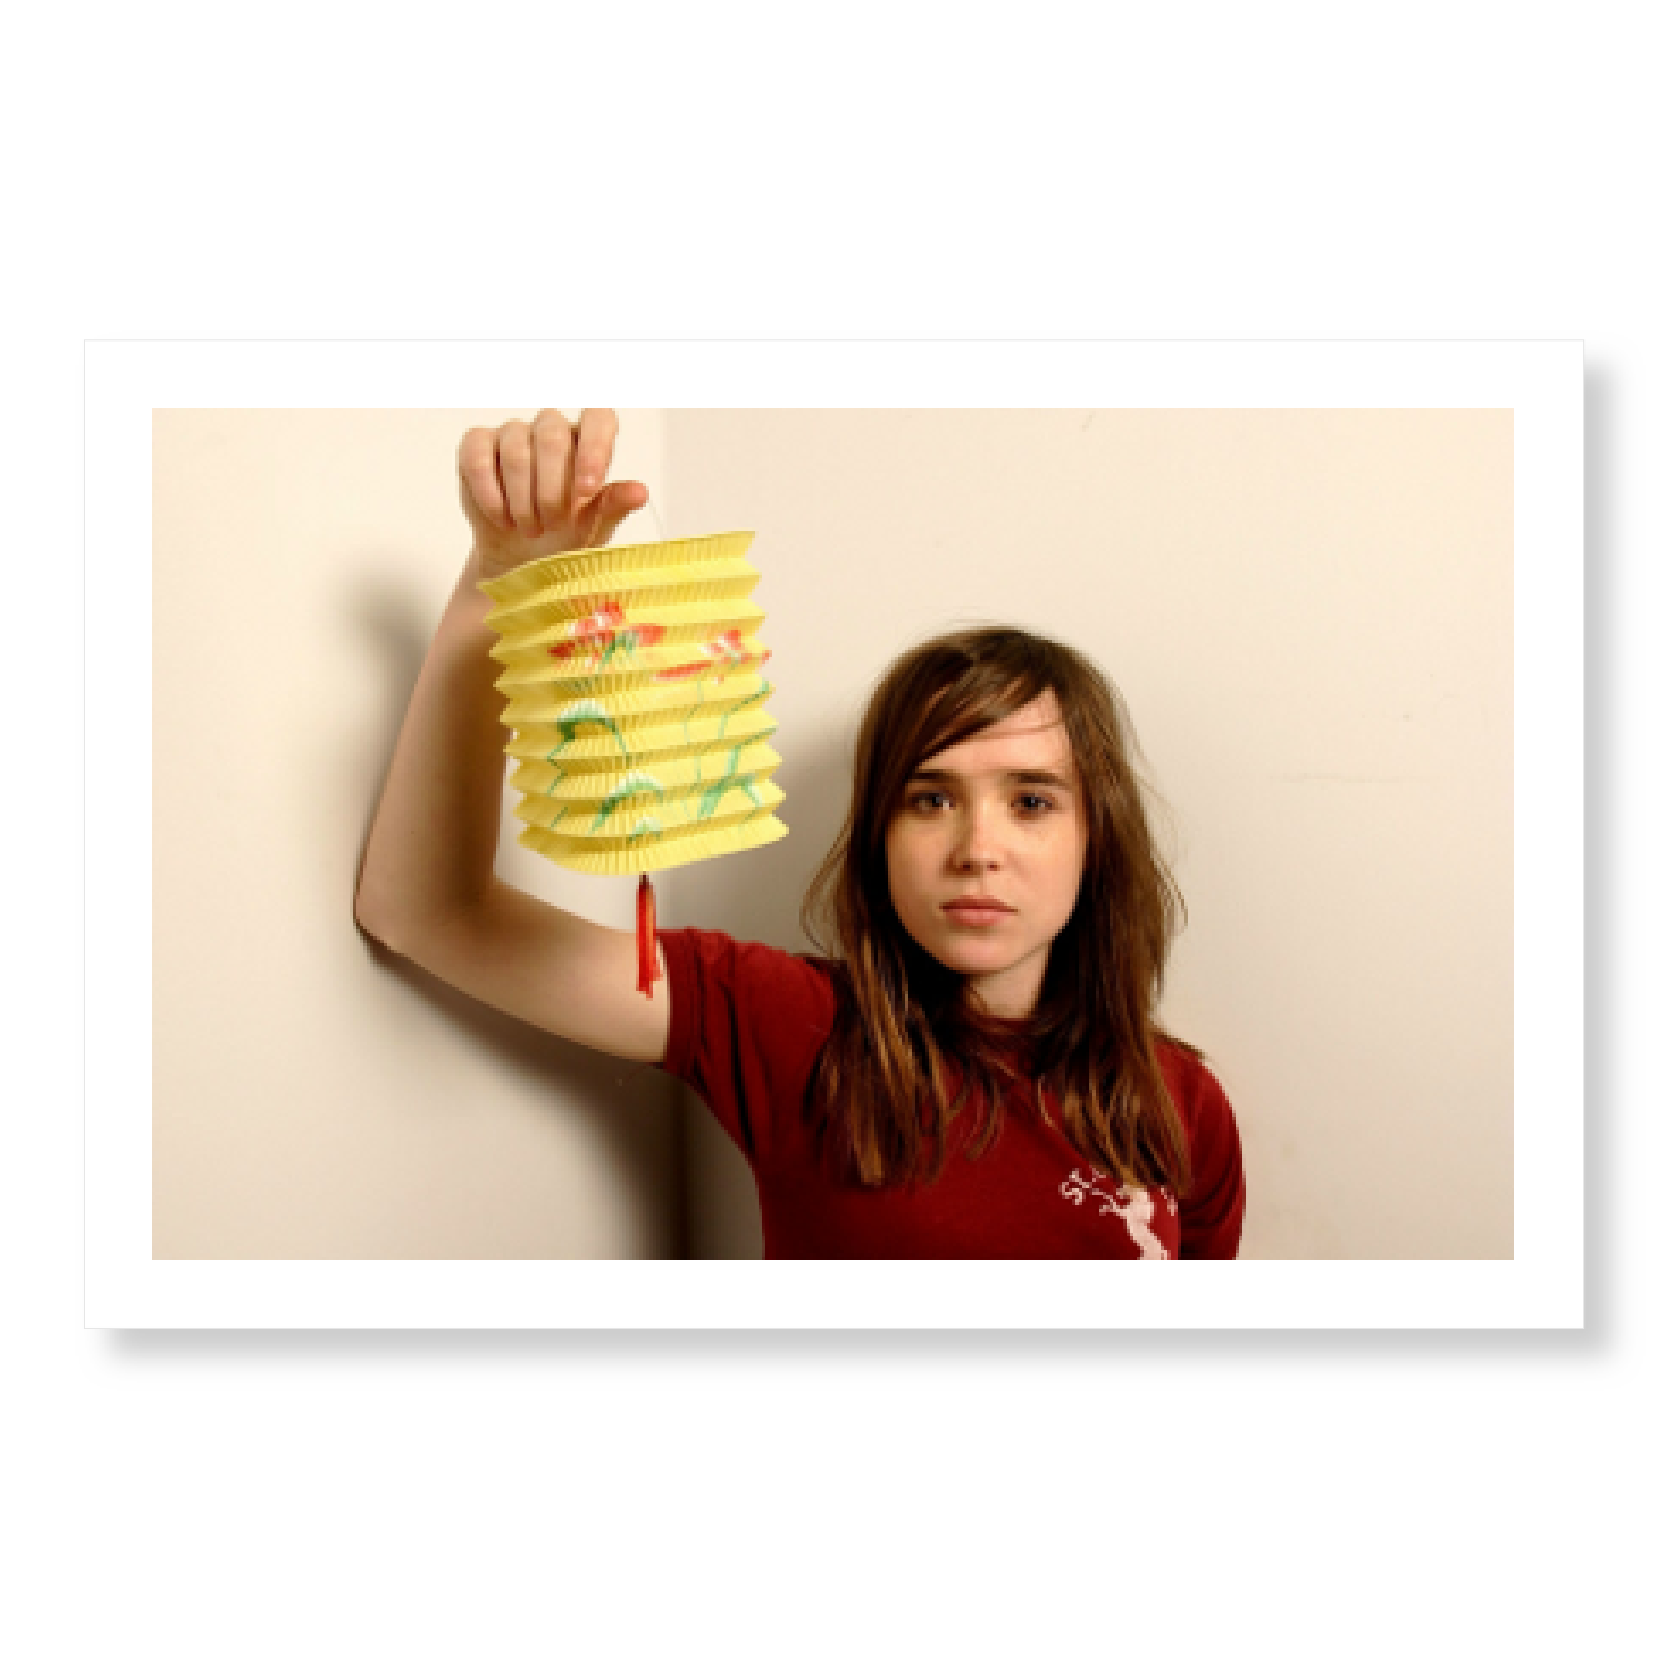
\includegraphics[height=.2\textwidth]{penma/schaubild/sample_file.pdf}
%	\pause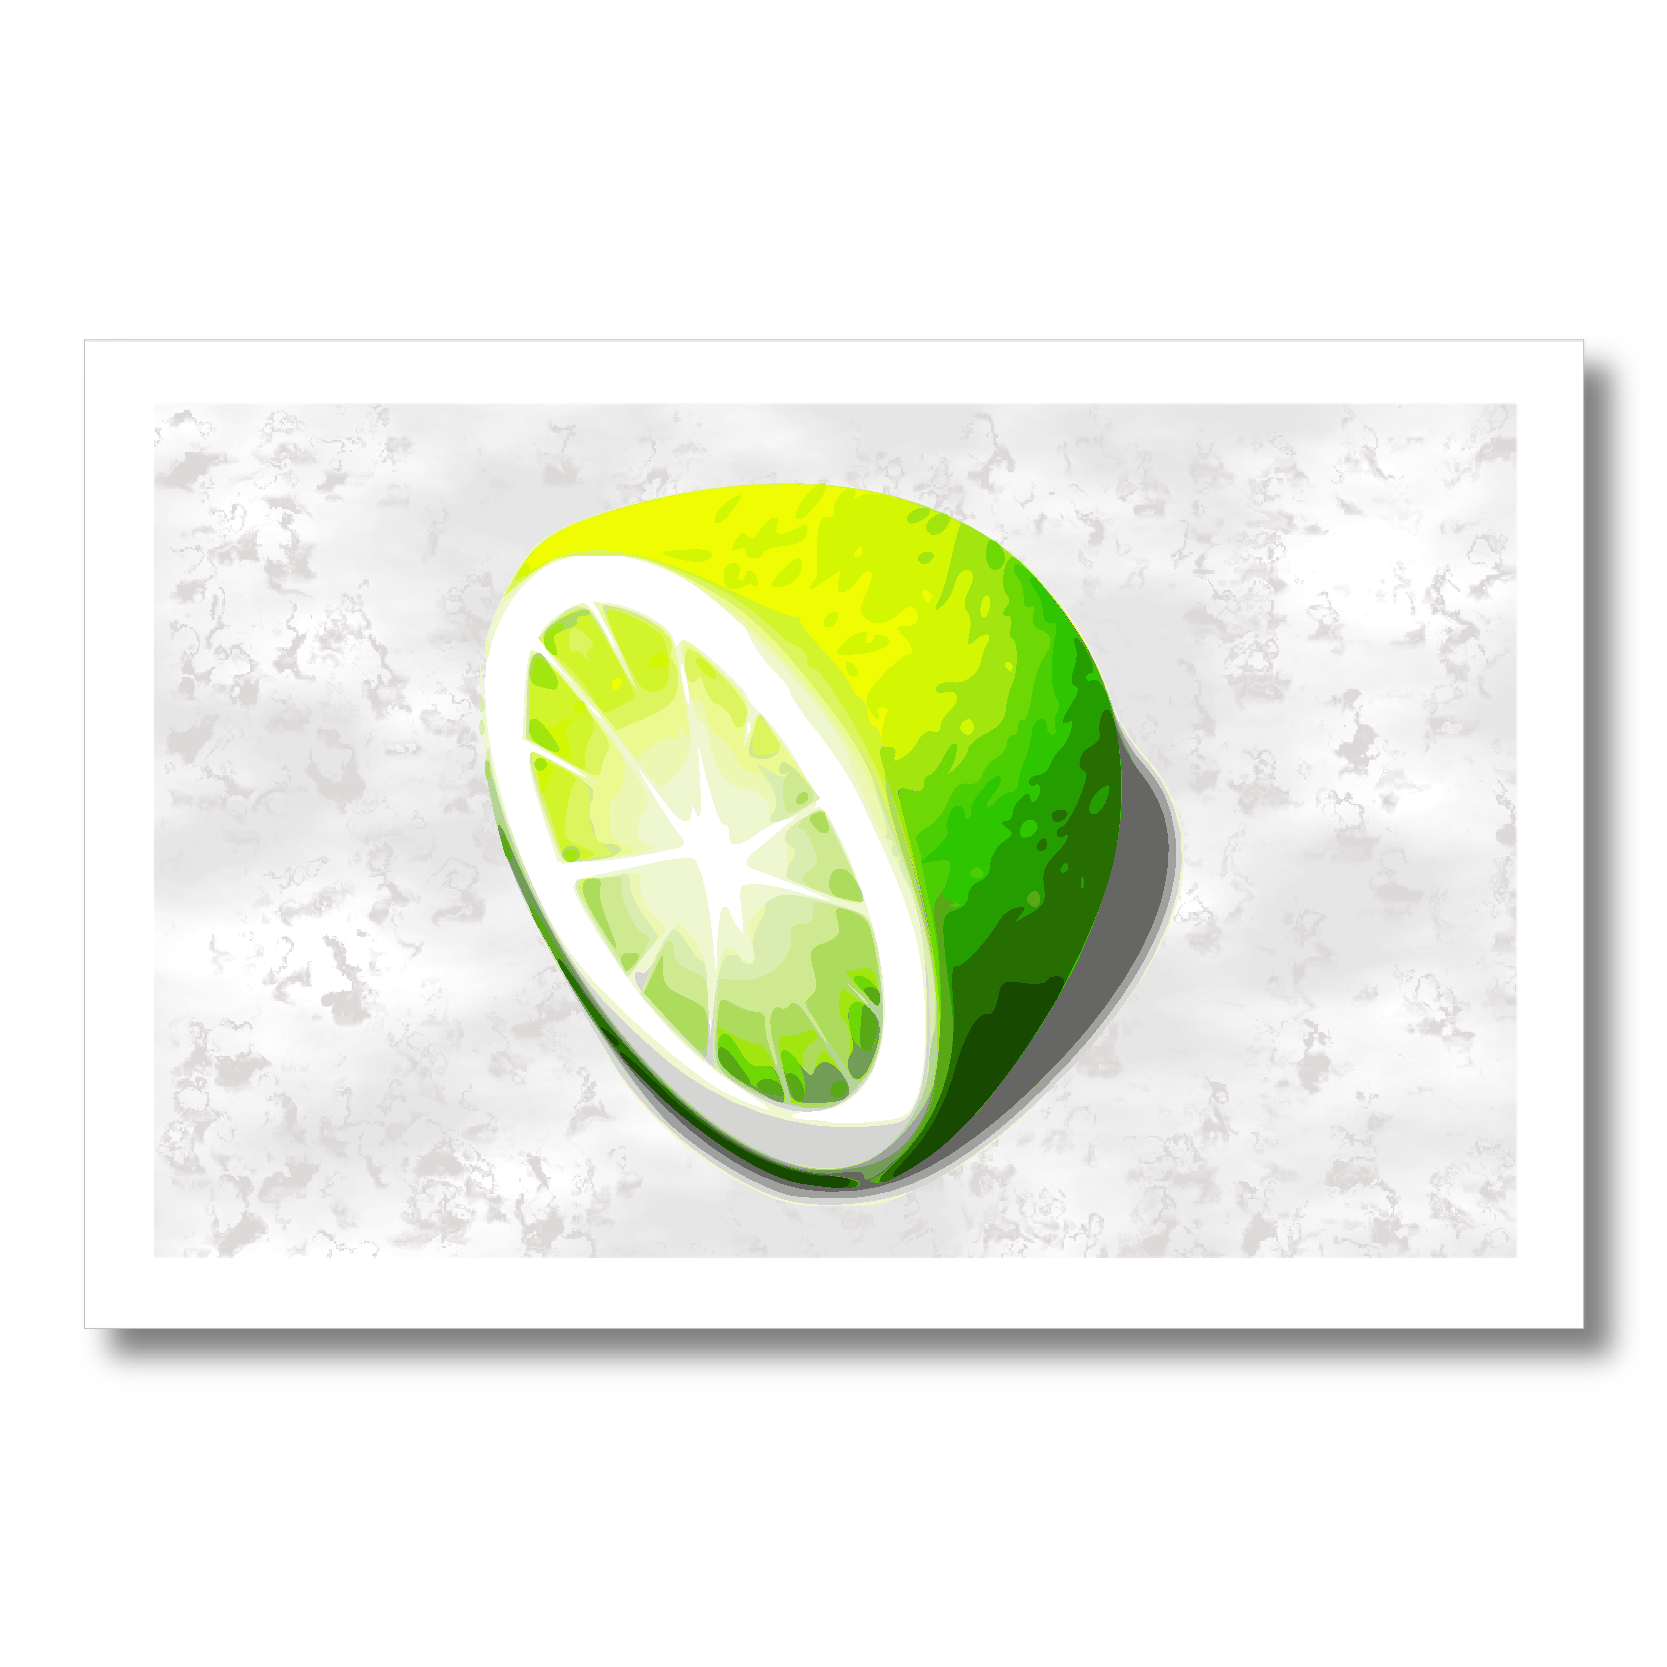
\includegraphics[height=.2\textwidth]{penma/schaubild/sample_file_ALT.pdf}
	\pause
\includegraphics[height=.2\textwidth]{penma/schaubild/pfeil.pdf}
	      
\includegraphics[height=.2\textwidth]{penma/schaubild/dpaper.pdf}
	\pause
\includegraphics[height=.2\textwidth]{penma/schaubild/pfeil.pdf}
	      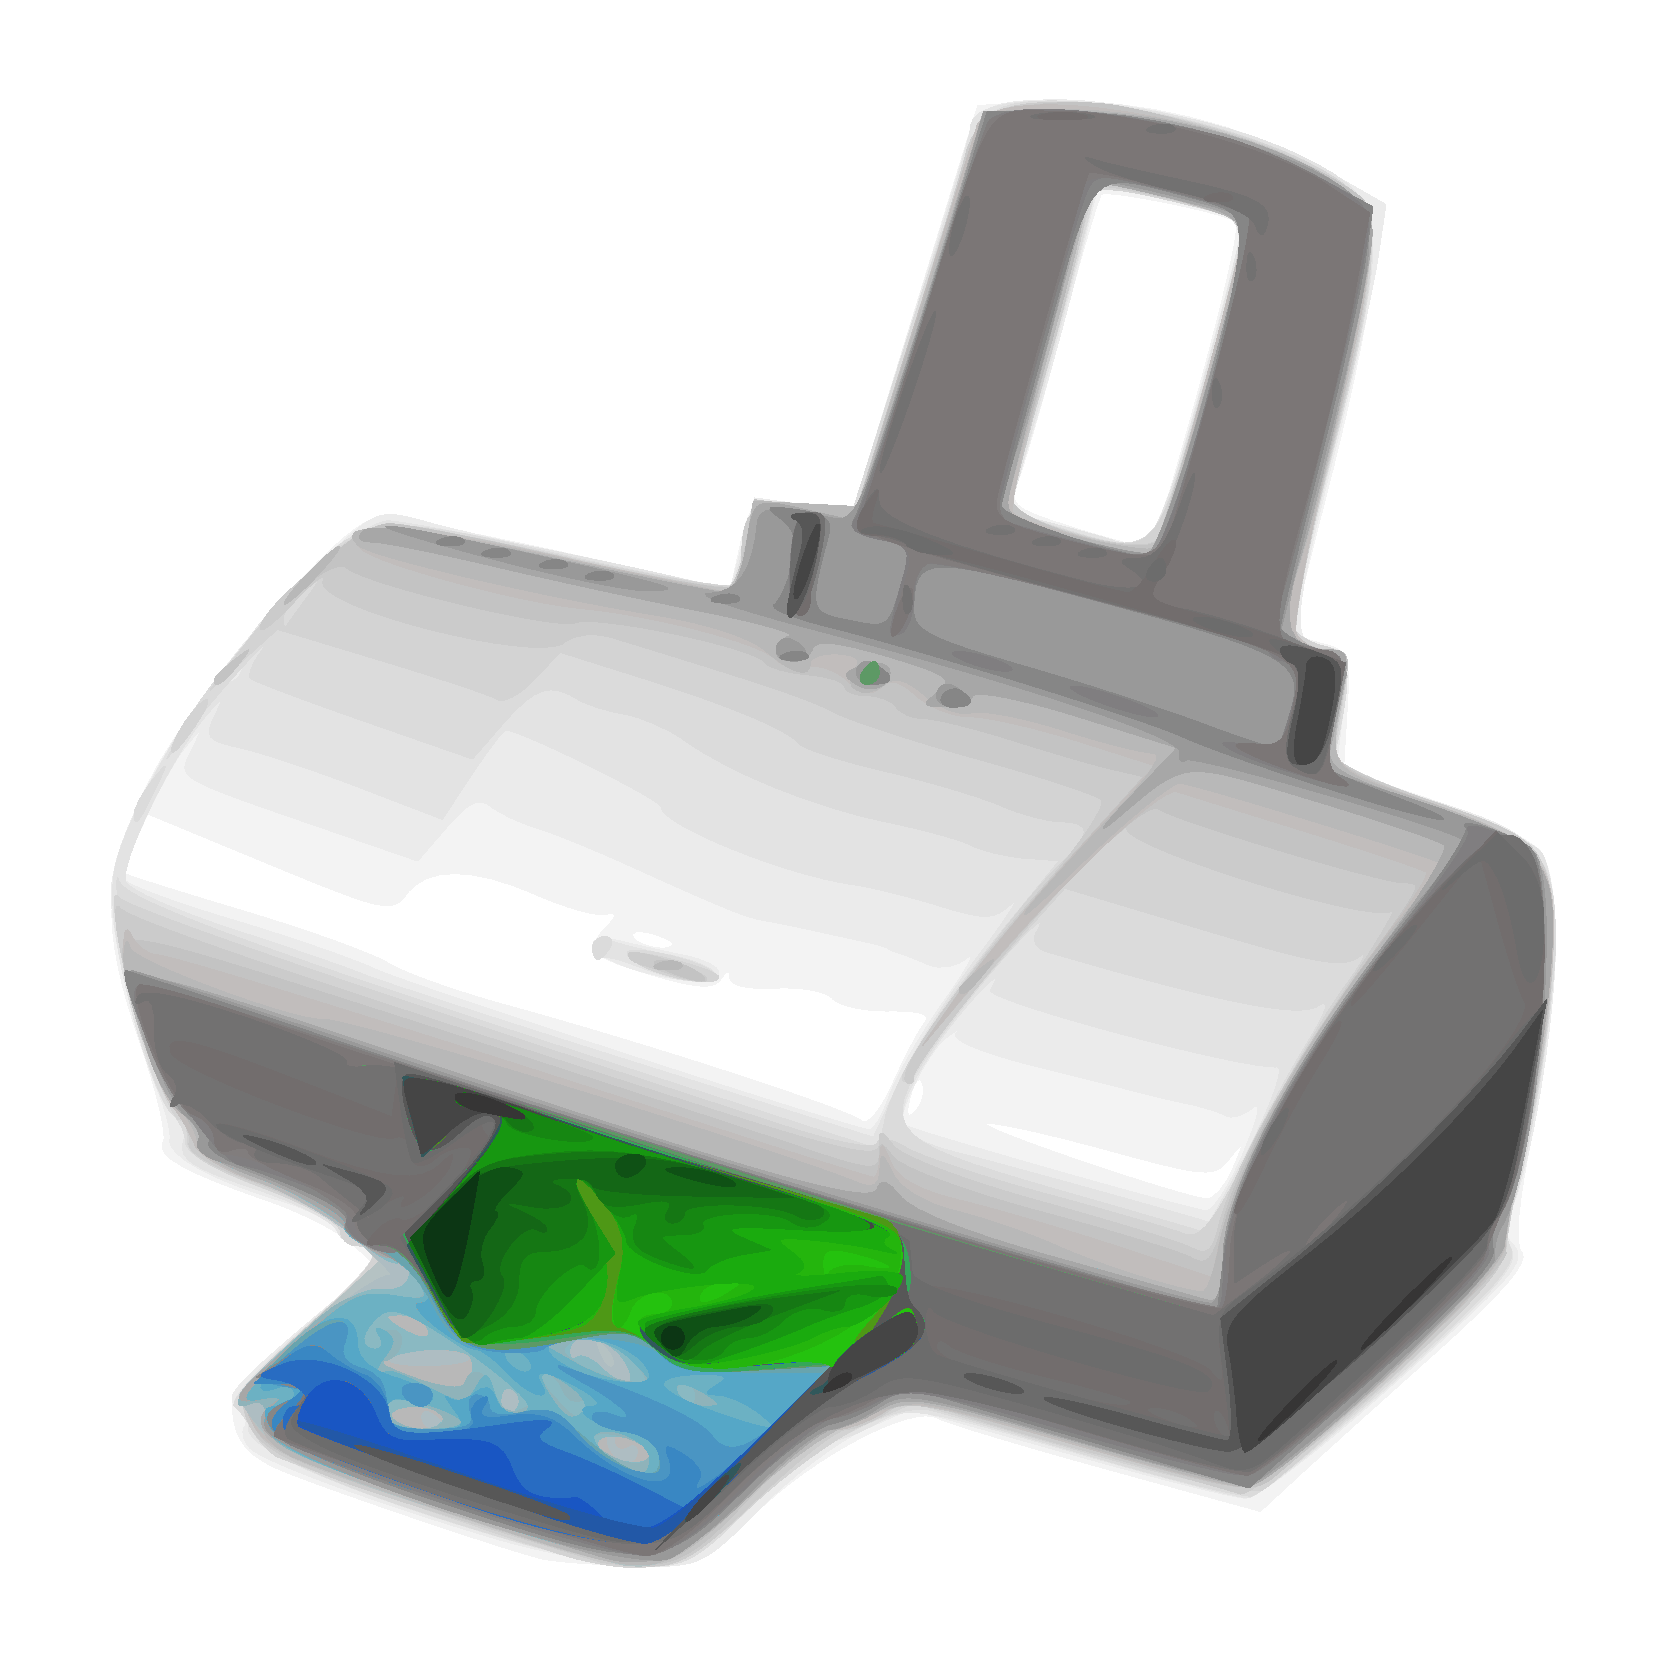
\includegraphics[height=.2\textwidth]{penma/schaubild/printer.pdf}
	\pause
\includegraphics[height=.2\textwidth]{penma/schaubild/pfeil.pdf}
	      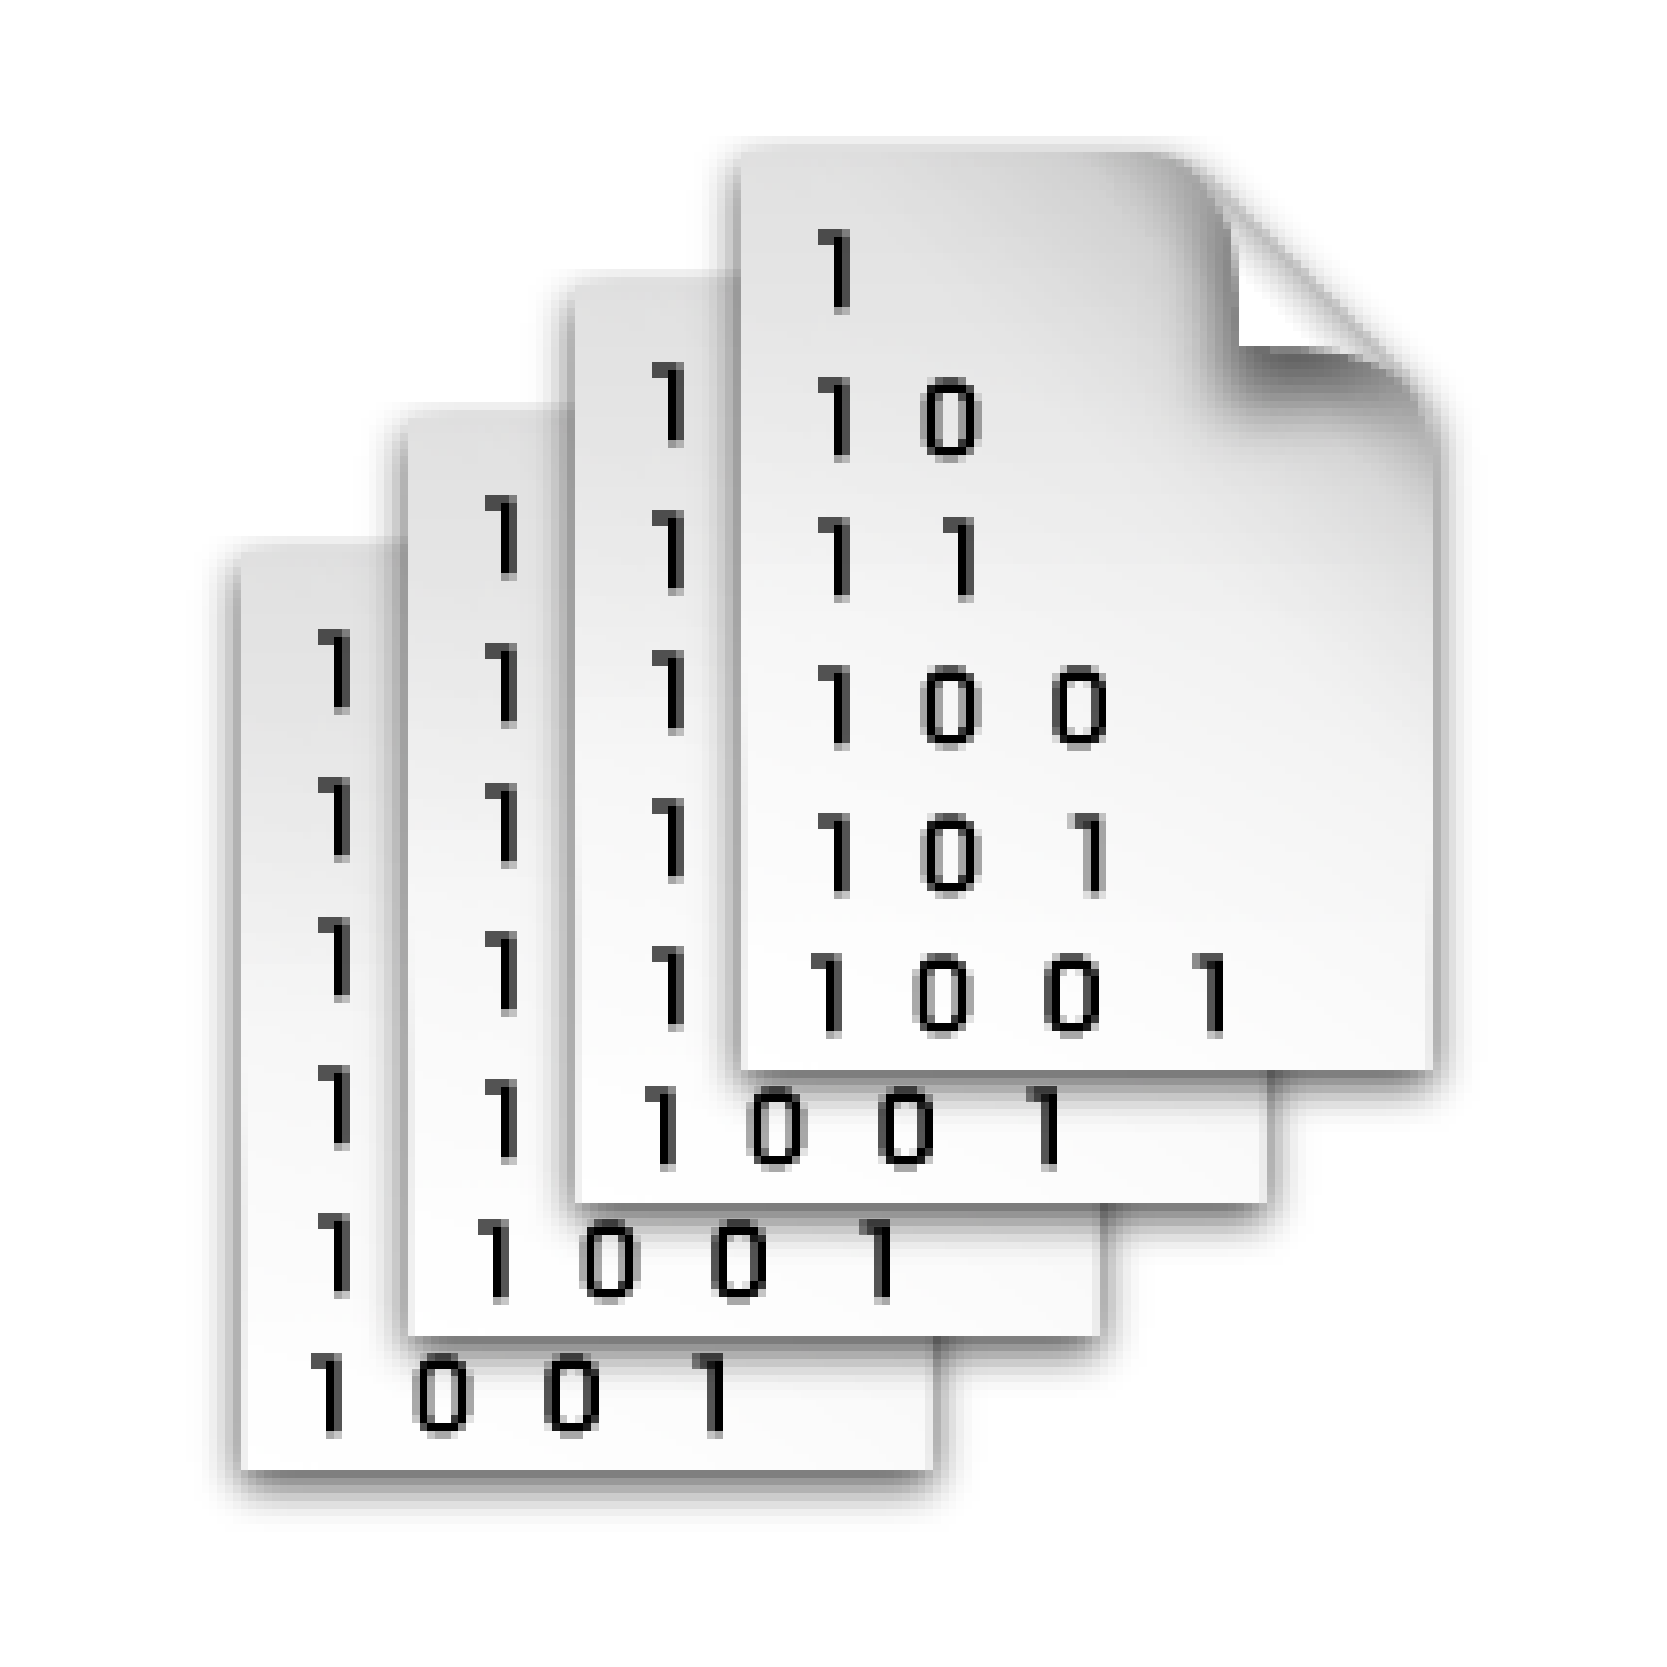
\includegraphics[height=.2\textwidth]{penma/schaubild/binary_documents.pdf}
	\vspace{1em}
	\pause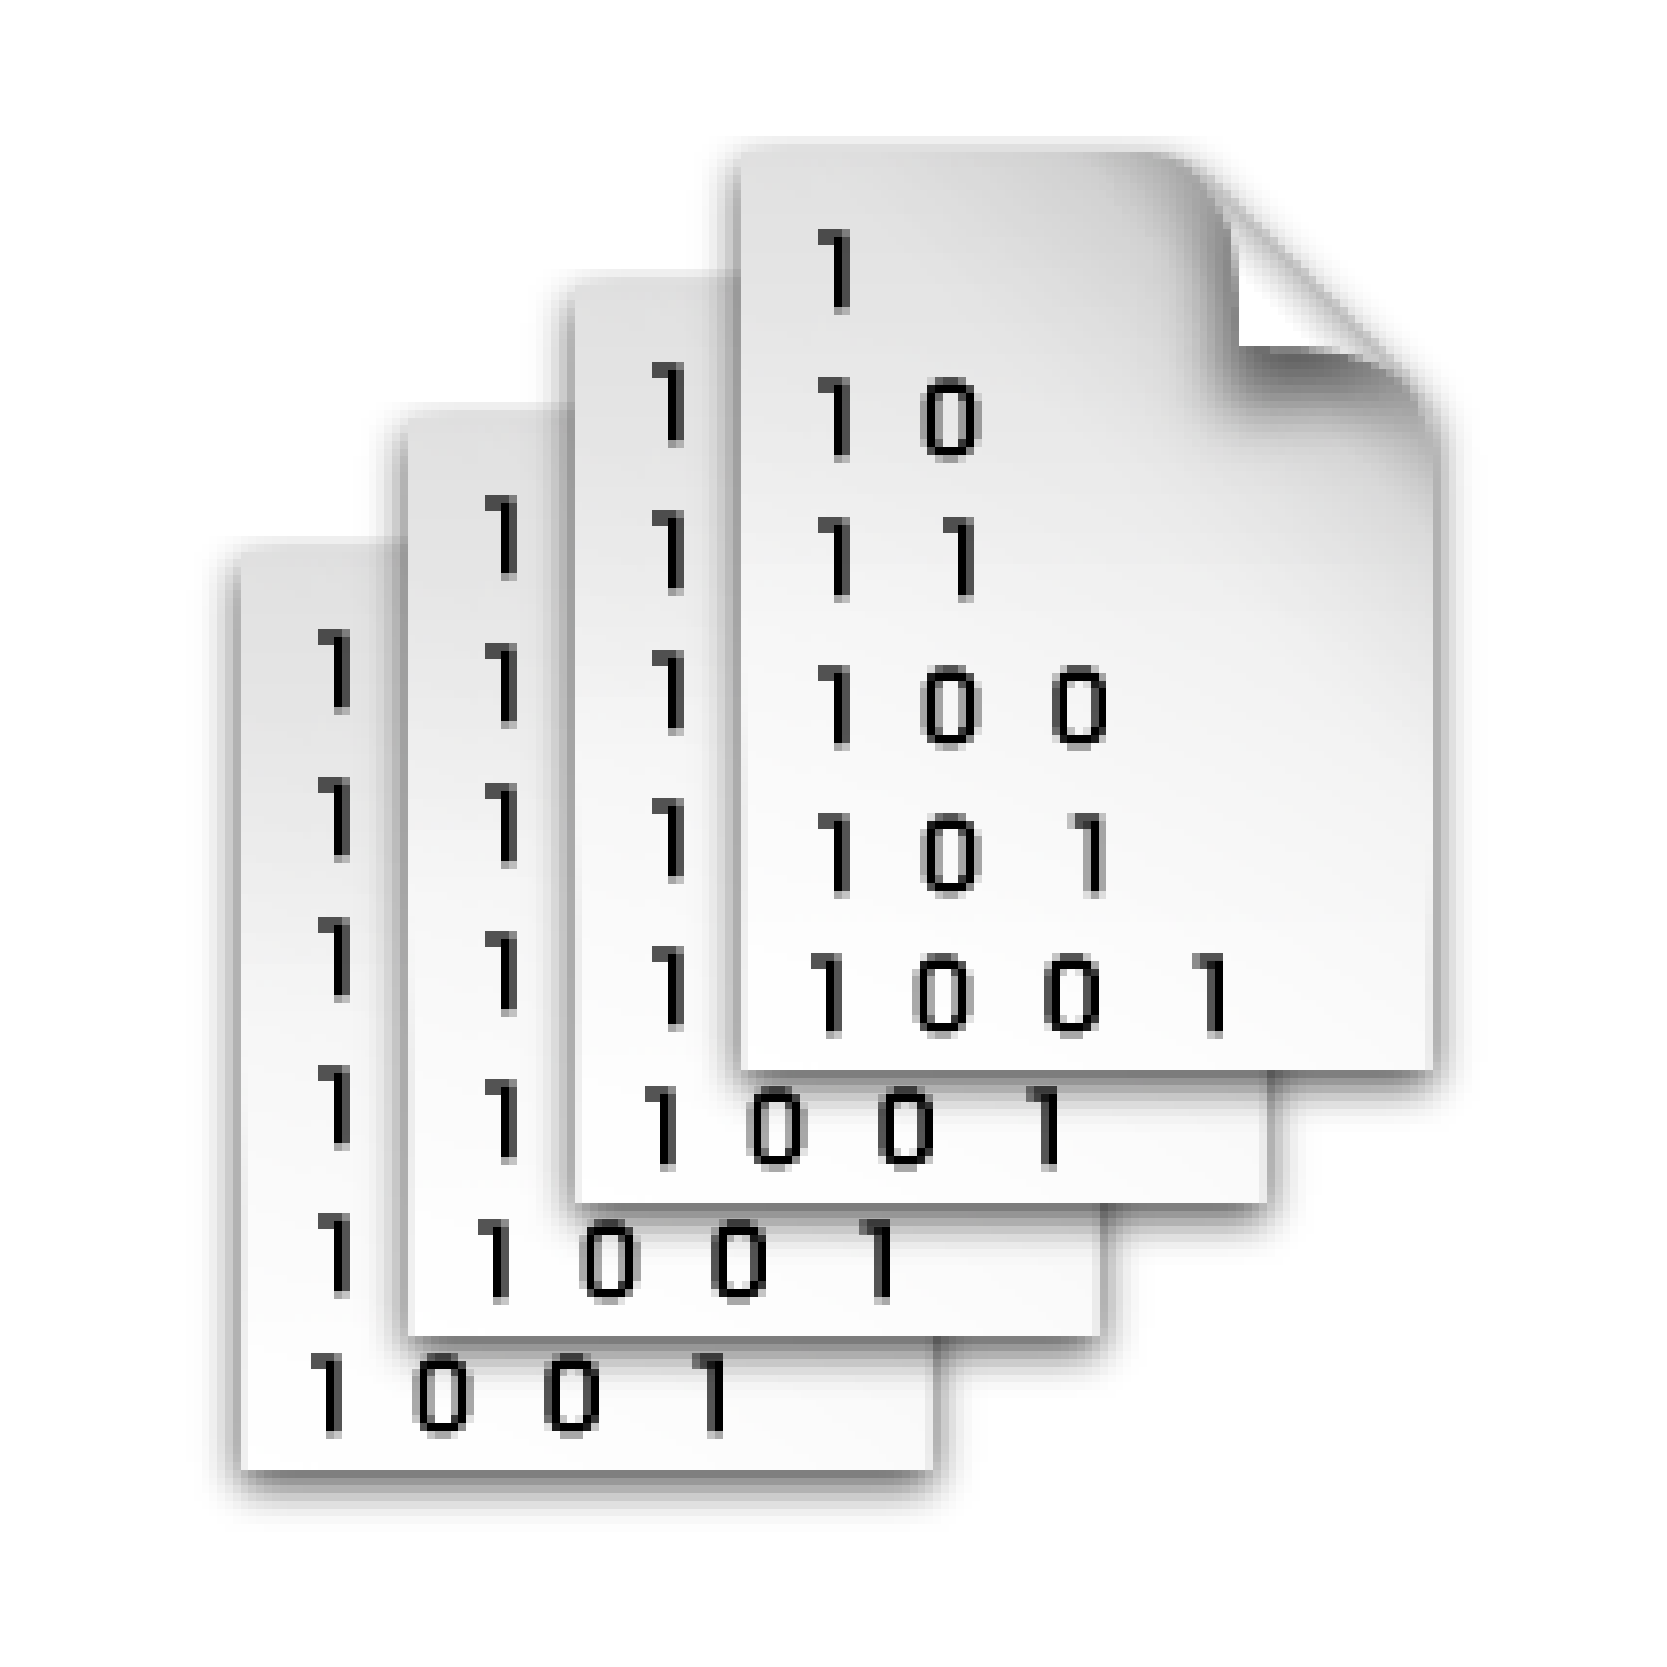
\includegraphics[height=.2\textwidth]{penma/schaubild/binary_documents.pdf}
	\pause
\includegraphics[height=.2\textwidth]{penma/schaubild/pfeil.pdf}
	      
\includegraphics[height=.2\textwidth]{penma/schaubild/scanner.pdf}
	\pause
\includegraphics[height=.2\textwidth]{penma/schaubild/pfeil.pdf}
	      
\includegraphics[height=.2\textwidth]{penma/schaubild/dpaper.pdf}
	\pause
\includegraphics[height=.2\textwidth]{penma/schaubild/pfeil.pdf}
	      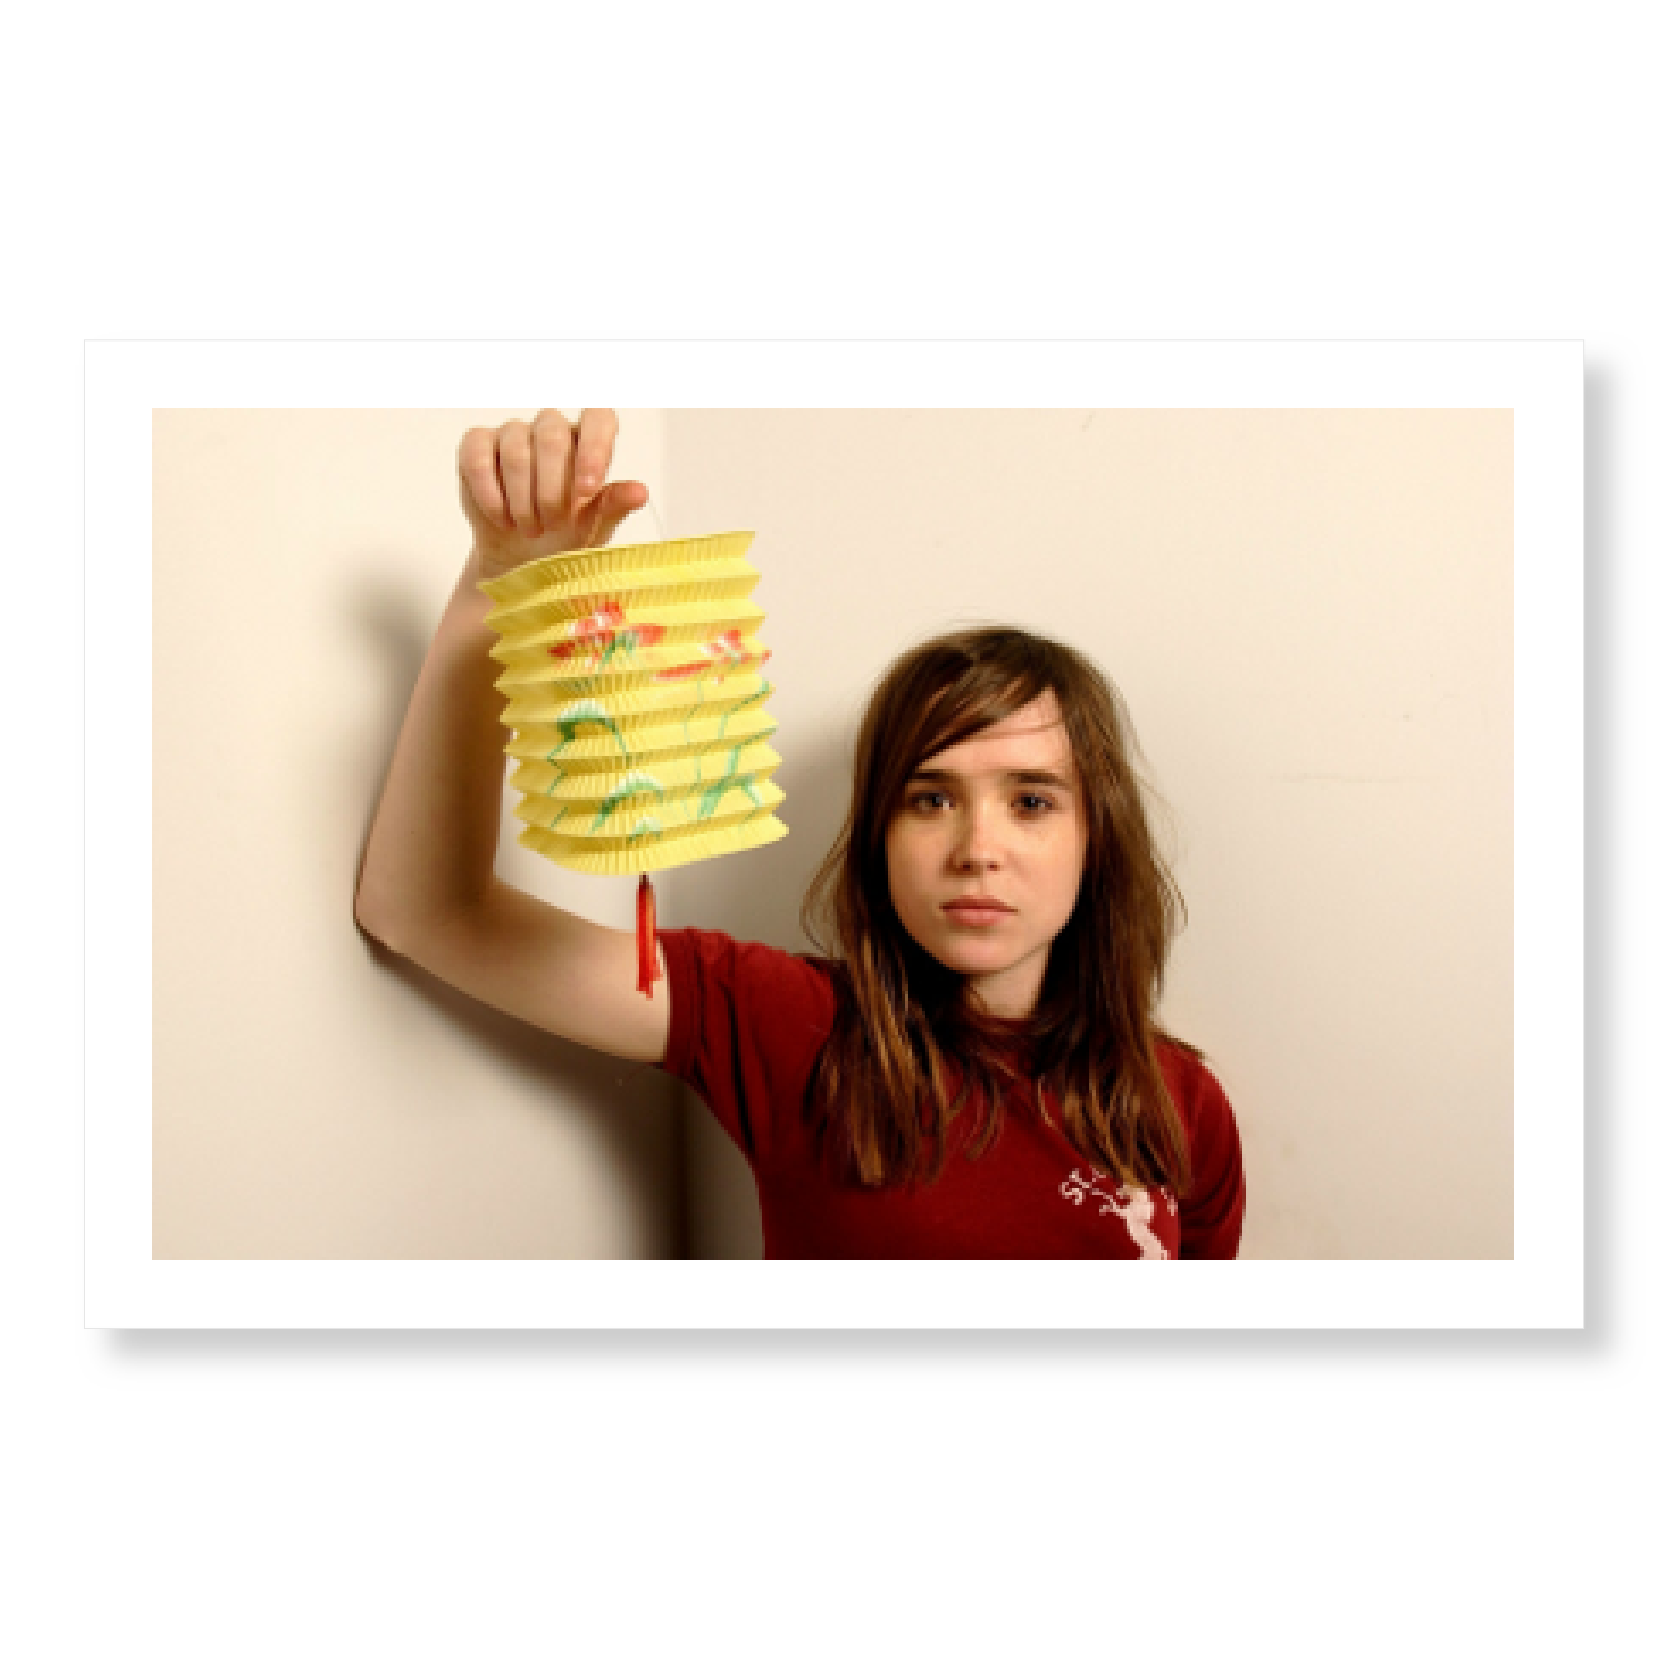
\includegraphics[height=.2\textwidth]{penma/schaubild/sample_file.pdf}
%	      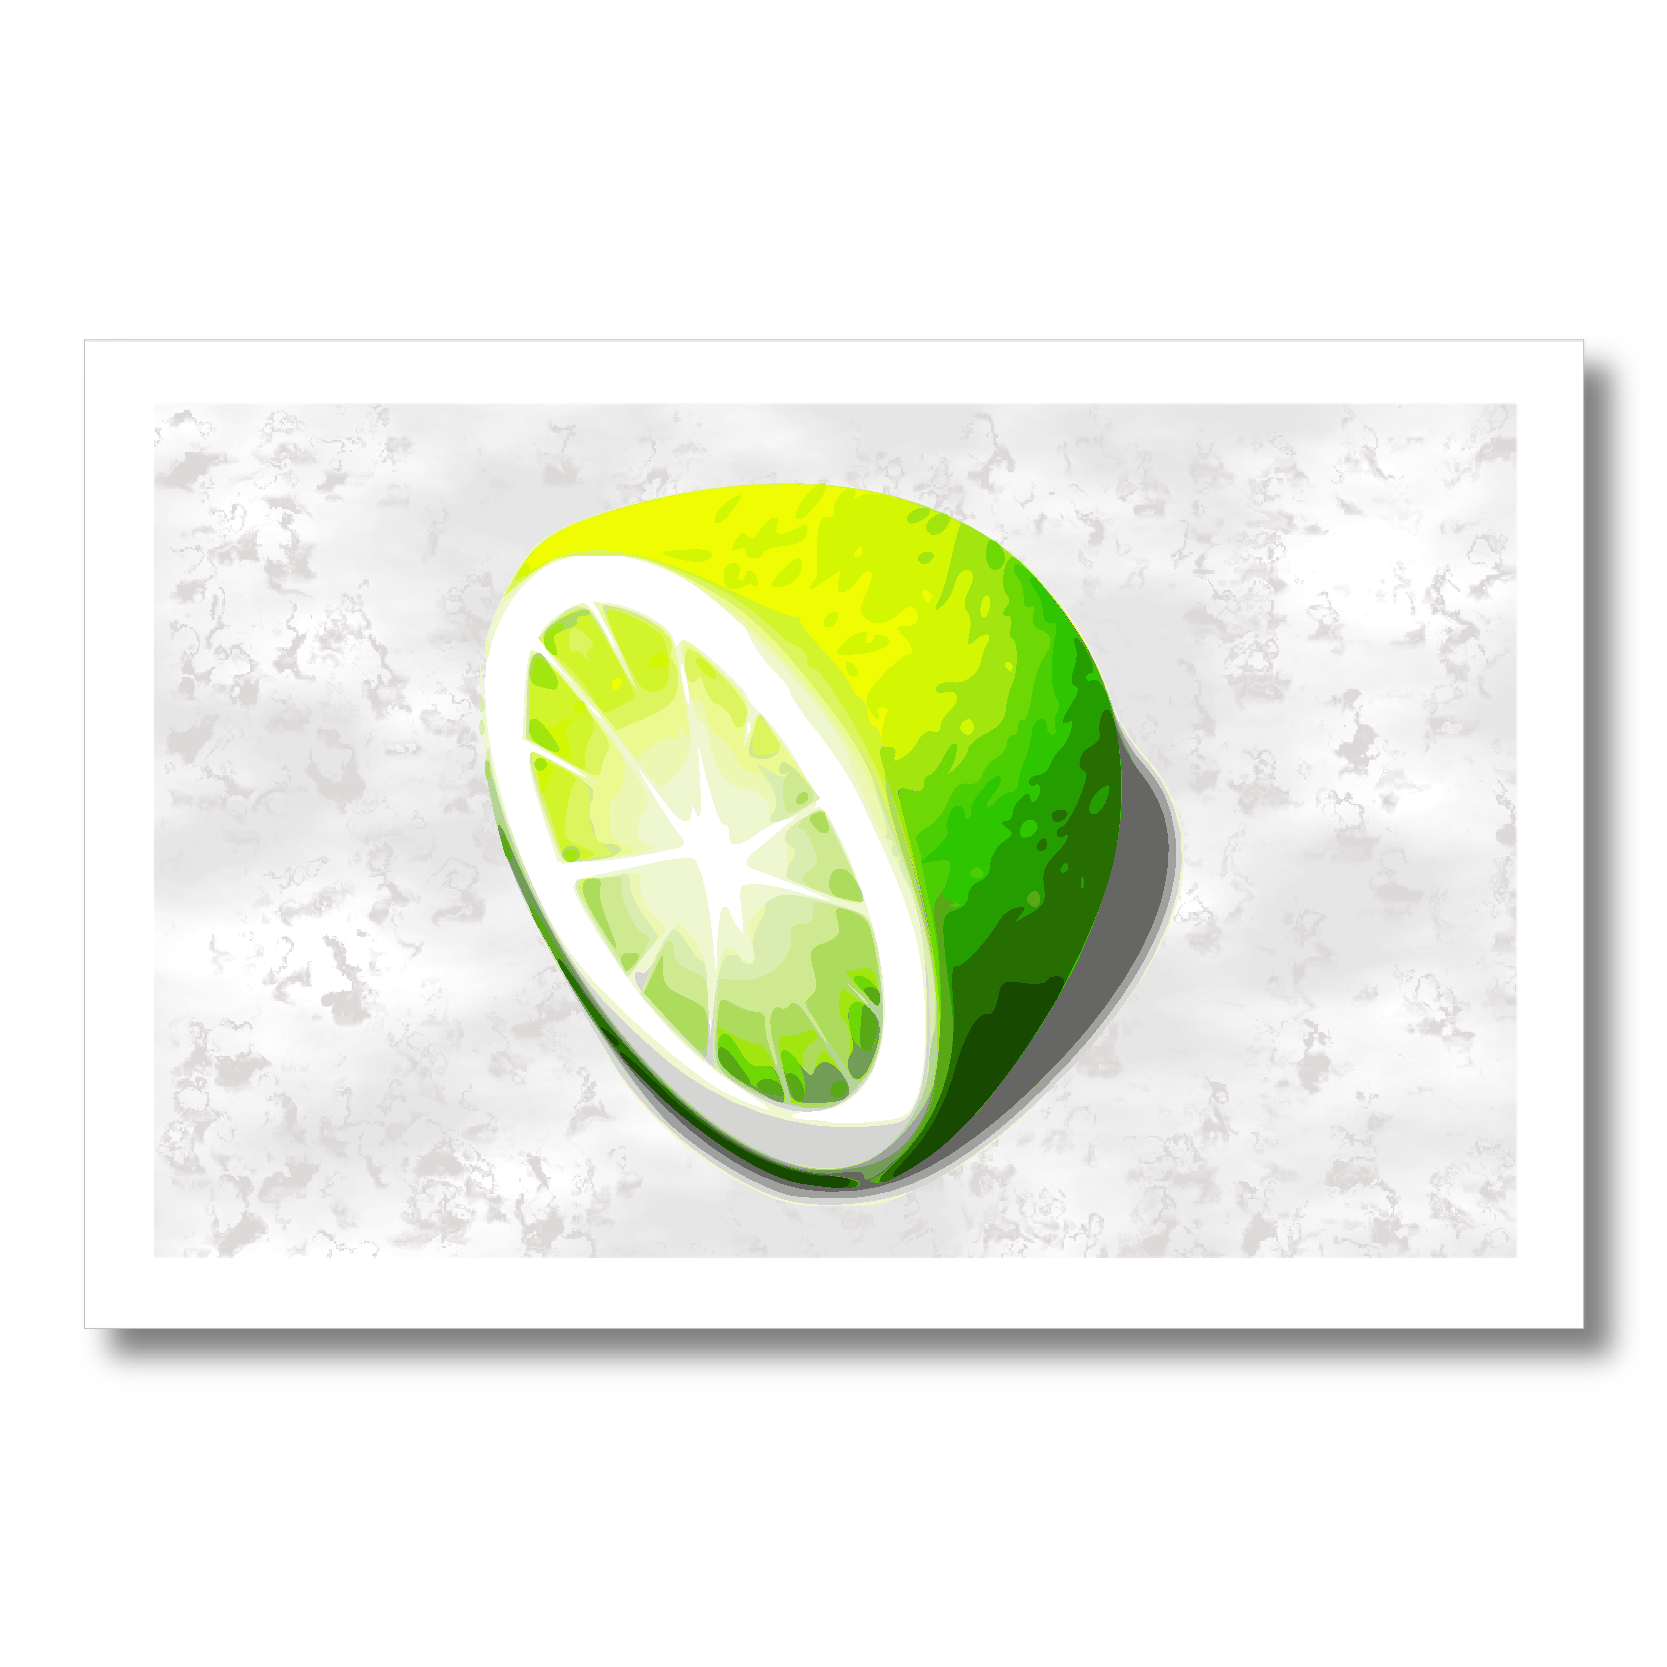
\includegraphics[height=.2\textwidth]{penma/schaubild/sample_file_ALT.pdf}
\end{frame}

\subsection{Mögliche Speicherformate}
\begin{frame}{Mögliche Speicherformate}
	\begin{itemize}
	\item Text + Zeichenerkennung
	\item 2D-Codes (QR-Code, DataMatrix)
	\item Barcodes
	\end{itemize}
\end{frame}

\section{OCR-A}

\subsection{OCR-A im Jahr 1968}
\begin{frame}{OCR-A im Jahr 1968}
	\begin{columns}
	\column{.65\textwidth}
		\begin{itemize}
		\item<2-> Schrift aus der Frühzeit der optischen Zeichenerkennung
		\item<3-> Sieht scheiße aus
		\item<4-> Die Kisten der 70er konnten es lesen
		\end{itemize}
	\column{.35\textwidth}
		\onslide+<1->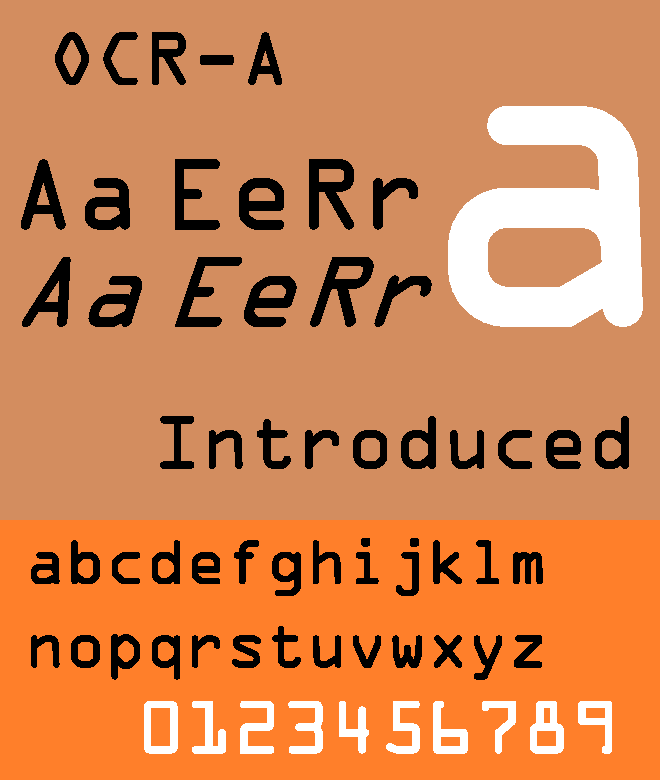
\includegraphics[width=\textwidth]{penma/others/ocr-a.pdf}
	\end{columns}
\end{frame}

\subsection{OCR-A im Jahr 2010}
\begin{frame}{OCR-A im Jahr 2010}
	\begin{columns}
	\column{.5\textwidth}
		\onslide+<2->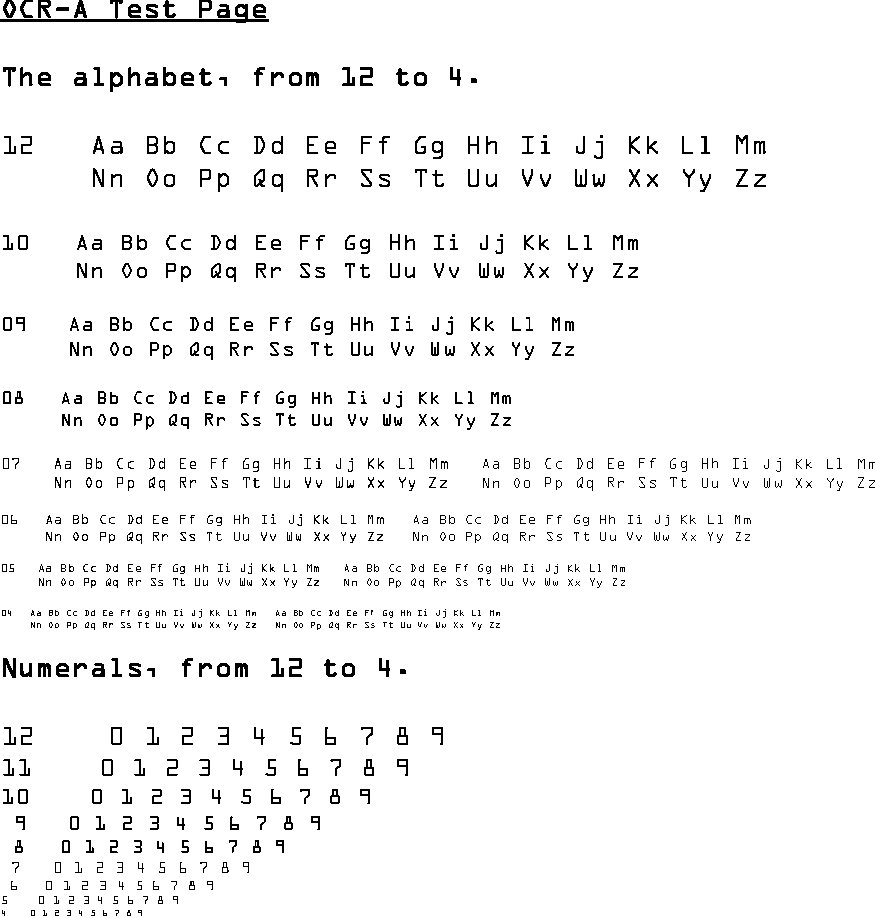
\includegraphics[width=\textwidth]{penma/gocr/testdoc.pdf}
	\column{.5\textwidth}
		\onslide+<3->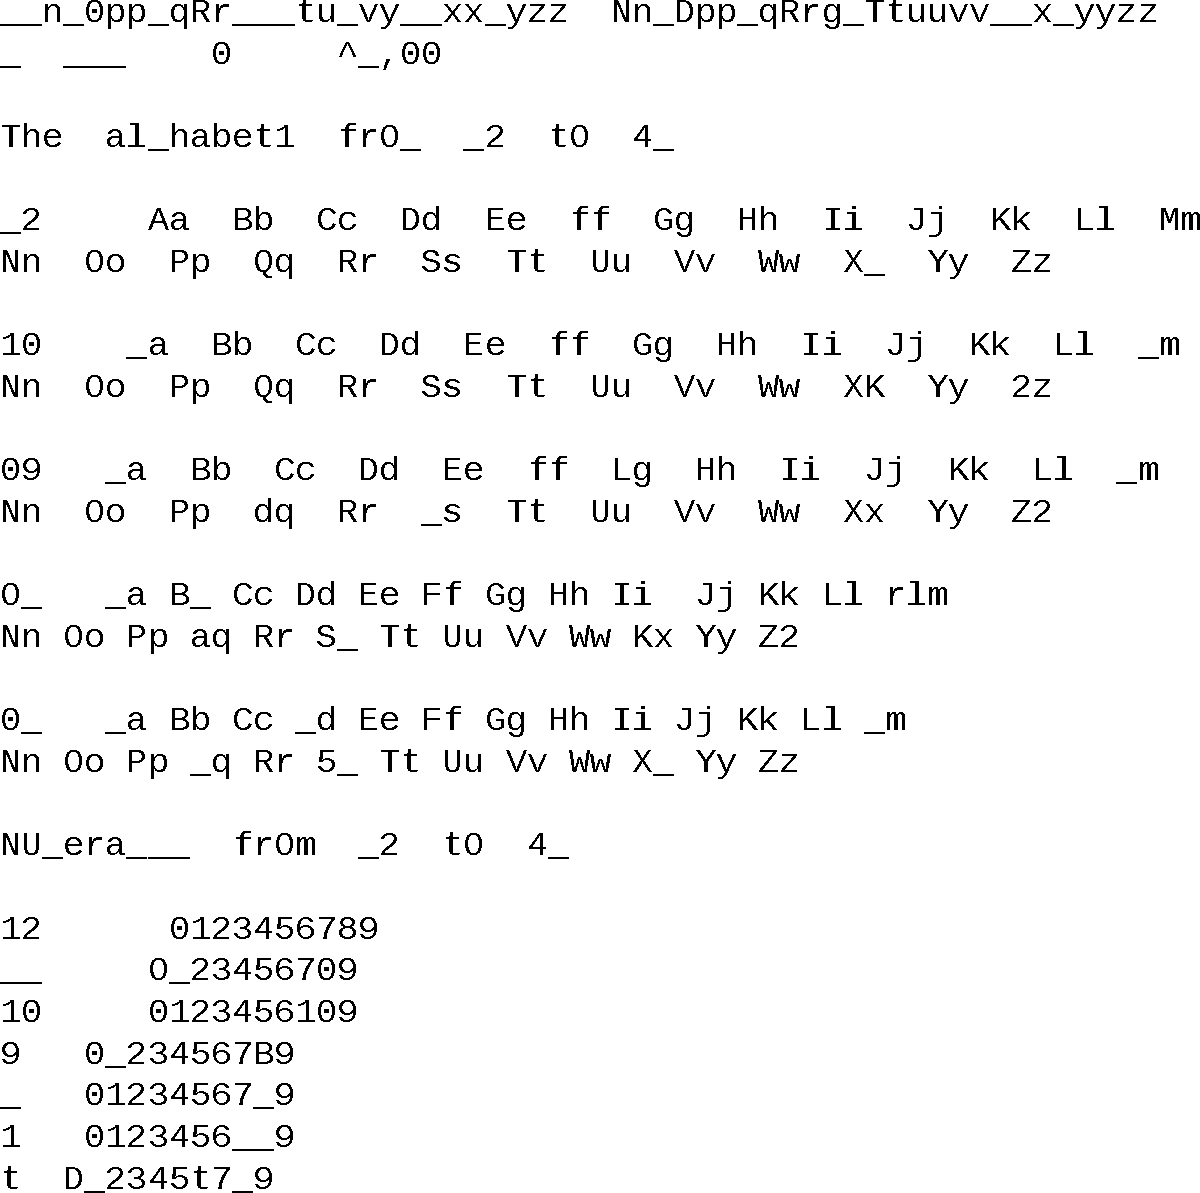
\includegraphics[width=\textwidth]{penma/gocr/readout-t.pdf}
	\end{columns}
\end{frame}

\begin{frame}[<+->]{OCR-A im Jahr 2010}
	\begin{itemize}
	\item Nicht einmal OCR-A wird richtig erkannt
	\item Auch nicht mit sehr großer Schrift
	\item Dabei war es nur ein Screenshot
	\item Ein Test mit Scan scheiterte komplett
	\end{itemize}
\end{frame}

\begin{frame}{OCR-A im Jahr 2010}
	\begin{columns}
	\column{.65\textwidth}
		\begin{itemize}
		\item<+-> 16 Zeichen können recht fehlerfrei unterschieden werden: \\ \texttt{AaDdEeHhTtRrYy2347}
		\item<+-> Mit kleinstmöglicher Schriftgröße ca. 5700 Byte pro Seite
		\item<+-> Und 20 manuell zu behebenden Lesefehlern
		\end{itemize}
	\column{.35\textwidth}
		\onslide+<+->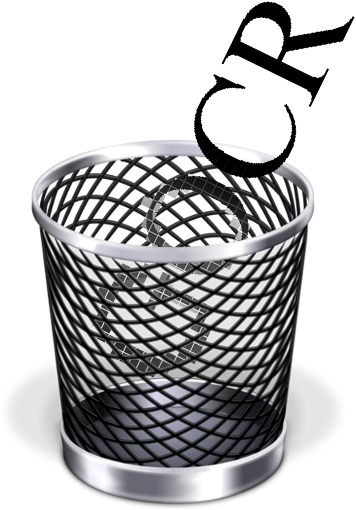
\includegraphics[width=\textwidth]{penma/trashcans/gocr.png}
	\end{columns}
\end{frame}

\section{2D-Codes}

\begin{frame}{QR-Code und andere 2D-Geschichten}
	\begin{columns}
	\column{.65\textwidth}
		\begin{itemize}
		\item<2-> Zweidimensional
		\item<3-> Bietet Fehlerkorrektur
		\item<4-> Weitere Vorteile von muzy
		\item<5-> Maximale Datenmenge:
			\begin{itemize}
			\item QR-Code: ca. 3 KiB/Code
			\item DataMatrix: ca. 1.5 KiB
			\item Pro Seite 10 bis 20 KiB
			\end{itemize}
		\end{itemize}
	\column{.35\textwidth}
		\onslide+<1->
\includegraphics[width=\textwidth]{penma/codes/qr-chaosdorf.png}
	\end{columns}
\end{frame}

\begin{frame}{QR-Code und andere 2D-Geschichten}
	\begin{columns}
	\column{.65\textwidth}
		\begin{itemize}
		\item<+-> Freie Dekodiertools verfügbar
		\item<+-> Erkennen aber größere Codes nicht richtig
		\item<+-> Funktionieren auch bei minimalen Bildfehlern (Scan) nicht richtig
		\item<+-> Zu unzuverlässig für Datenspeicherung
		\end{itemize}
	\column{.35\textwidth}
		\onslide+<4->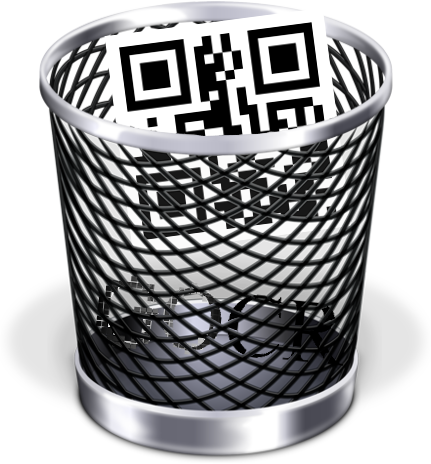
\includegraphics[width=\textwidth]{penma/trashcans/qr.png}
	\end{columns}
\end{frame}

\section{Barcodes}

\begin{frame}{Barcodes}
	\begin{columns}
	\column{.65\textwidth}
		\begin{itemize}
		\item<1-> Speichern vergleichsweise wenig Daten pro Code
		\item<2-> Lassen sich aber gut stapeln
		\item<3-> Beispiel: PDF417 (gestapelte 1D-Codes)
		\item<4-> Aber keine freie Lesesoftware
		\item<5-> Also normale Codes selbst stapeln
		\end{itemize}
	\column{.35\textwidth}
		\onslide+<1->
\includegraphics[width=\textwidth]{penma/codes/128-chaosdorf.pdf}
		\vspace{1em}
		\onslide+<3->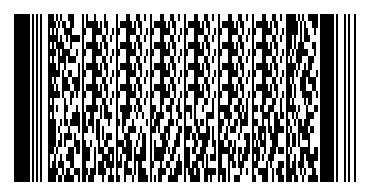
\includegraphics[width=\textwidth]{penma/codes/417.png}
	\end{columns}
\end{frame}

\subsection{ZBAR}
\begin{frame}{ZBAR}
	\begin{columns}
	\column{.75\textwidth}
		\begin{itemize}
		\item<1-> Für 1D-Codes gibt es gute Software
		\item<2-> ZBAR <\texttt{http://zbar.sf.net}>
		\item<3-> Erkennt viele Barcode-Typen
		\item<4-> Gute Erkennungsrate auch bei schlechten Scans
		\end{itemize}
	\column{.25\textwidth}
		\onslide+<2->
\includegraphics[width=\textwidth]{penma/others/zbar.pdf}
	\end{columns}
\end{frame}

\subsection{Erster Versuch mit gestapelten Codes}
\begin{frame}{Erster Versuch mit gestapelten Codes}
	\begin{columns}
	\column{.65\textwidth}
		\begin{itemize}
		\item<2-> Rechts: Anhäufung von Code128-Barcodes
		\item<3-> ZBAR liest Codes in zufälliger Reihenfolge aus
		\item<4-> Enthält darum Nummer des Datenblocks
		\item<5-> 3840 Byte pro Seite
		\end{itemize}
	\column{.35\textwidth}
		\onslide+<1->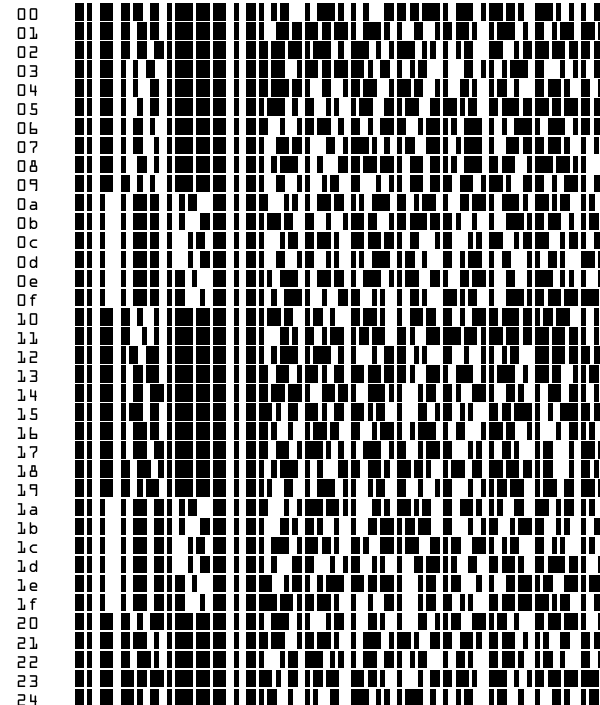
\includegraphics[width=\textwidth]{penma/outputs/simple_stack.png}
	\end{columns}
\end{frame}

\subsection{Fehlerkorrektur}
\begin{frame}[<+->]{Fehlerkorrektur}
	\begin{itemize}
	\item Etwa 90\% aller Codes werden ohne weiteres erkannt
	\item Der Rest müsste aufwendig nachbearbeitet werden
	\item Weitere Gefahr: teilzerstörte Dokumente (Staub, Flecken, Risse, ...)
	\item Lösung: Vorwärtsfehlerkorrektur
	\item Nun \emph{4800} Byte in \emph{160} Zeilen
		\begin{itemize}
		\item Aber weiterhin nur 3840 Byte Nutzdaten
		\end{itemize}
	\end{itemize}
\end{frame}

\subsection{Weitere Optimierungen}
\begin{frame}{Weitere Optimierungen}
	\begin{itemize}
	\item<1-> Verteilung auf zwei Spalten
		\begin{itemize}
		\item<2-> Weniger nicht erkannte Codes
		\end{itemize}
	\item<3-> Erhöhung der Datenmenge auf 4096 Byte pro Seite
	\item<4-> Hinzufügen eines Seitenheaders (Name, Offset, Länge)
	\end{itemize}
	\onslide+<5->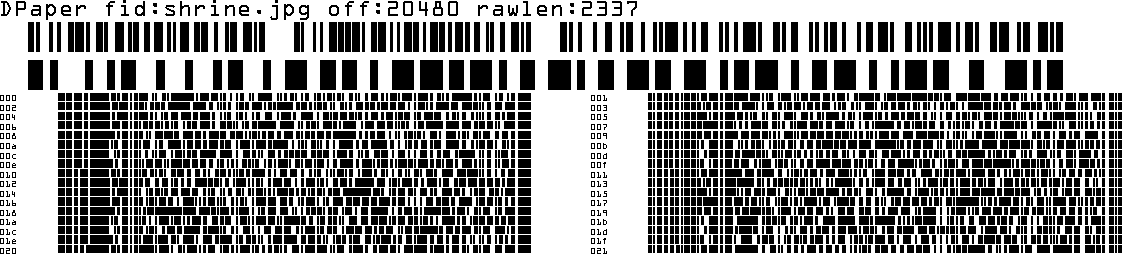
\includegraphics[width=\textwidth]{penma/outputs/current_t.pdf}
\end{frame}

\section{Anwendung}

\begin{frame}[fragile]{Anwendung}
	\small\begin{semiverbatim}
% ./encode_file -I foo2.jpg < foo.jpg \pause
% lpr output.ps \pause

% while true; do scanimage | ./decode_file; done
retrieved data from image!
... ^C \pause
% diff -s foo.jpg foo2.jpg
Files foo.jpg and foo2.jpg are identical
\end{semiverbatim}
\end{frame}

\section{Abschluss}

\subsection{Nachteile von Papier als Speichermedium}
\begin{frame}[<+->]{Nachteile von Papier als Speichermedium}
	\begin{itemize}
	\item Geringe Speicherdichte
	\item Für größere Datenmengen zu teuer
	\item Und zu langsam
	\item Büropapier und Druckertinte haben keine lange Lebensdauer
	\item Warum also auf Papier speichern?
	\item Because we can
	\end{itemize}
\end{frame}

\subsection{Fragen?}
\begin{frame}{Fragen?}
	\hfill\textbf{github.com/penma/dpaper}\hfill\hbox{}
\end{frame}

